\documentclass[10pt,twocolumn,letterpaper]{article}

% cvpr.sty pulls in xcolor itself, so the table option has to be passed to it
% rather than requested a second time.
\PassOptionsToPackage{table}{xcolor}
\usepackage{cvpr}              % camera-ready

% cvpr.sty requests Times but silences font warnings, and the bold weight was
% not being found: every \textbf in the body rendered as regular. newtxtext
% supplies a complete Times family, so bold is bold.
\usepackage{newtxtext}
\usepackage{graphicx}
\usepackage{amsmath}
\usepackage{amssymb}
\usepackage{booktabs}
\usepackage[shortlabels]{enumitem}
\usepackage[pagebackref,breaklinks,colorlinks]{hyperref}
\usepackage[capitalize]{cleveref}
\crefname{section}{Sec.}{Secs.}
\Crefname{section}{Section}{Sections}
\Crefname{table}{Table}{Tables}
\crefname{table}{Tab.}{Tabs.}
\crefname{figure}{Fig.}{Figs.}

\def\cvprPaperID{*****}
\def\confName{CVPR}
\def\confYear{2026}

\newcommand{\code}[1]{\texttt{\small #1}}

% This template's \paragraph renders run-in headings in the body face, so they
% are invisible as headings. \textbf does produce a bold face here, so the
% run-in headings are set explicitly.
\newcommand{\runin}[1]{\par\smallskip\noindent\textbf{#1}\enspace}

\begin{document}

\title{TwinWorld 2026 Challenge Final Verification Factsheet\\
       Sparse-View 2D Gaussian Splatting with Corrected Depth Readout,\\
       and Optimal Covering Lattices for a Precision-Free Semantic Metric}

\author{An Kai Chen\\
National Tsing Hua University\\
{\tt\small kylechen.ankai@gmail.com}
}
\maketitle

%---------------------------------------------------------------------------
\section{Team details}

\begin{itemize}\itemsep2pt
\item \textbf{Team name:} \code{kylechen1211}
\item \textbf{Team leader:} An Kai Chen, National Tsing Hua University,
      \href{mailto:kylechen.ankai@gmail.com}{\tt kylechen.ankai@gmail.com}
\item \textbf{Rest of the team:} None; this is a single-member entry.
\item \textbf{Team website:} None.
\item \textbf{Codabench user name:} \code{kylechen1211}, identical to the team
      name for unambiguous identification.
\item \textbf{Codabench ID of the final submission:} \textbf{909861}, final
      phase, submitted 2026-08-31 09:56~UTC, archive
      \code{submission\_v0.30\_bcc019.zip}.
\item \textbf{Final challenge score:} \textbf{1.534}. Peak signal-to-noise
      ratio (PSNR) 19.95, structural similarity index measure (SSIM) 0.723,
      learned perceptual image patch similarity (LPIPS) 0.290, F-score 0.582,
      mean intersection over union in 3D (mIoU 3D) 0.341; equivalently
      \code{rendering\_score} 0.610, \code{geometry\_score} 0.582,
      \code{semantic\_score} 0.341.
\item \textbf{Source code, checkpoints and factsheet:}
      \url{https://github.com/kylevirtuous1211/ECCV-TwinWorld-challenge}
\item \textbf{Complete results in the native representation:}
      \url{https://drive.google.com/drive/folders/1423PRQBWKVaPb3fDJeUy4nV5z5sJklMf}
\end{itemize}

%---------------------------------------------------------------------------
\section{Method details}

\subsection{Overall pipeline}

\Cref{fig:pipeline} summarizes our pipeline. We build on 2D Gaussian
Splatting (2DGS)~\cite{huang2024_2dgs}, implemented with
gsplat~\cite{gsplat}. The submission pipeline introduces no additional network,
external data, or pretrained weights. Most of the performance gain comes from
three modifications, each evaluated on the six scenes with released ground
truth before inclusion in the final system.

\begin{figure*}[t]
\centering
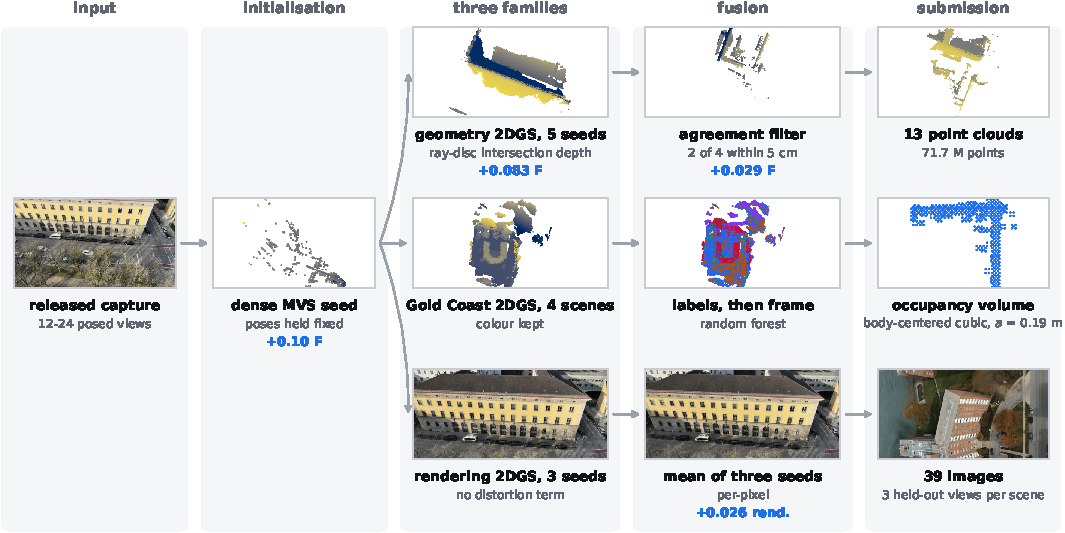
\includegraphics[width=\textwidth]{fig/pipeline.pdf}
\caption{Overview of the pipeline. A common dense initialization is used to
train three families of Gaussian models: TUM geometry (five seeds with agreement
filtering), Gold Coast geometry (also providing color features to the semantic
classifier), and rendering (three seeds with per-pixel averaging). The occupancy volume
in the submission column is described in \cref{sec:disclosure}. Gains shown in blue are measured on the six scenes with
released ground truth.}
\label{fig:pipeline}
\end{figure*}

\runin{1. A dense multi-view stereo (MVS) seed.}
The released sparse reconstruction covers only 0.07--0.20\% of
image pixels and appears to be cropped from a larger model: all reprojection
errors are zero, and the image identifiers fall in the 700--800 range although the
model contains at least 819 images. We replace this initialization: we densely
re-triangulate the released images with the released poses held fixed, then run
COLMAP~\cite{schoenberger2016colmap} dense MVS. This change improves
F-score by 0.10 on the held-out scenes.

\runin{2. Exposing and correcting the 2DGS depth rule.}
Because 2DGS represents surfaces as oriented discs, depth varies across each
projected footprint and must be evaluated at the ray--disc intersection. The
native gsplat path instead passes center depth as a per-Gaussian color channel,
assigning a constant depth across the footprint. We recover the intersection
depth from the
outputs an unmodified gsplat installation already returns, so no change to the
CUDA kernels is needed. On identical checkpoints from four TUM scenes,
this correction improves \code{geometry\_score} from \textbf{0.3888 to 0.4717}
and produces point clouds with 7--11\% fewer points.

\runin{3. Averaging three rendering seeds.}
Rendering quality varies across random seeds, but selecting the best seed
requires ground truth, which is unavailable for the final-phase scenes. We
instead train three models per scene and average their outputs per pixel. This
improves \code{rendering\_score} by 0.026 over the single seed that would
otherwise have been submitted, and by 0.021 over the \emph{best} of the three
seeds on the released scenes. The same selection-free procedure applies directly
to the held-out scenes. \Cref{fig:renders} shows the result against the released
reference images on three scenes, and what averaging does not fix.

\subsection{Extra data}

\textbf{No.} All inputs are drawn from the released \code{TwinWorld\_Datasets}
(Hugging Face snapshot \code{8d5dfff}) or from the scores returned for our own
submissions. We use no external ground truth, data outside the challenge release,
or pretrained scene reconstructions. The only pretrained weights used anywhere
in our experiments are those of the VGG network inside the reference LPIPS
implementation. It is used only for local LPIPS evaluation, not in any
submission.

We do use the ground truth the organisers released. The label classifier is
trained on it: every training label is taken from the nearest point of the
released ground-truth clouds of \code{scene\_009} and \code{scene\_010}, which
is what those two scenes ship them for. Two further uses, in which development-set ground
truth informs predictions on scenes that ship none, are summarized in
\cref{sec:disclosure}.

\subsection{Training strategy}

We train separate models for geometry and rendering because the two objectives
favor different configurations.

\runin{Geometry.}
Nine TUM scenes at five seeds each, and four Gold Coast scenes. 2DGS,
7000 iterations for TUM and 15{,}000 for Gold Coast, normal weight 0.05,
distortion weight 0.01, intersection-depth readout, and initialization from the
dense MVS seed. Seed~0 is fused into a point cloud, while seeds 1--4 are used
only for agreement filtering. A point from seed~0 is retained if at least two of
the other four seeds place a point within 5\,cm. On the four TUM scenes with
released ground truth, this filter improves \code{geometry\_score} from 0.4730
to 0.5016 ($+0.029$). It removes 49\% of points from the released-seed clouds on
which it was tuned and 28.5\% from the submitted dense-MVS clouds. This reduction
allows the submission to retain the full 2\,cm fusion resolution while remaining
within the evaluator's point budget.

\runin{Rendering.}
Thirteen scenes at three seeds each. We train 2DGS for 7000
iterations with a normal weight of 0.05, a distortion weight of 0, and the same
dense MVS initialization. The three outputs are averaged per pixel.

\runin{Semantics.}
We train a random forest~\cite{scikit-learn} with 200 trees,
a maximum depth of 32, and a minimum leaf size of 2. Its inputs comprise
geometric features and rendered color. The classifier is fitted to reconstructed
clouds rather than ground-truth clouds. In the corrected coordinate frame,
training on the reconstruction and including color jointly improve
\code{semantic\_score} by 0.15.

\runin{Frame correction.}
The released Gold Coast ground truth is displaced by
1.1--1.4\,m from the camera coordinate frame defined by its corresponding
images. This discrepancy originates in the released data rather than in our
reconstruction: registering the released sparse reconstruction directly to the
released ground-truth cloud, with nothing of ours involved, recovers the same
0.25\textdegree{} rotation. We measure this discrepancy on the two Gold Coast
scenes with released ground truth. As a control, the corresponding offsets on
the four TUM scenes range from 0.014 to 0.074\,m.

\subsection{Complexity and cost}

\Cref{tab:cost} gives the cost of one pass over the dataset.

\begin{table}[h]
\centering\small
\setlength{\tabcolsep}{4pt}
\begin{tabular}{@{}lrrr@{}}
\toprule
Model family & Scenes & Gauss. & Training \\
\midrule
Geometry, TUM, per seed & 9 & 19.1\,M & not logged \\
Geometry, Gold Coast & 4 & 28.7\,M & not logged \\
Rendering, per seed & 13 & 25.5\,M & 43\,min \\
\bottomrule
\end{tabular}
\caption{Cost of one pass over the dataset. Gaussians are summed over the scenes
in the row. Training wall clock was recorded per model only for the rendering
runs, whose receipts give 2.5 to 5.5 minutes each and 43 minutes for a seed over
all 13 scenes. The geometry runs timed only their fusion step, 45 to 1623
seconds per model with a mean of 283 over 49 models, so their training time is a
gap in our records rather than a small number.}
\label{tab:cost}
\end{table}

TUM geometry models contain 1.4--2.5\,M Gaussians per scene, and Gold Coast
models 7.0--7.5\,M. A rendering model trains in 2.5--5.5 minutes.
Rebuilding all 13 scenes takes approximately six hours on a single RTX~6000 Ada,
or two hours using a Slurm array on H200 nodes. A sampled geometry job used 7\,GB
of the available 48\,GB of graphics processing unit (GPU) memory. We train no
neural network beyond the
Gaussian representation, so a conventional parameter count does not apply. The
submitted archive contains 71.7\,M points across 13 point
clouds and 39 rendered images.

\subsection{Inference and submission}

No retraining is performed during submission generation. Geometry models are
rendered to depth maps, fused, agreement-filtered, and thinned. Gold Coast models
are assigned semantic labels and transformed to the corrected frame;
\code{scene\_011} and \code{scene\_012} are additionally converted to the
occupancy representation described in \cref{sec:disclosure}. Rendering outputs
are averaged across three seeds. The results bundle carries the complete
conversion procedure, command by command. Following it reproduces the two
submitted Gold Coast clouds byte for byte, and all 39 renders in the results bundle are byte-identical
to those in the submitted archive.

\subsection{Experimental results}

Our final score is 1.53, fourth among 21 entries in the closed final phase. Our
F-score of 0.58 is close to the challenge median of 0.57, whereas our
mIoU of 0.34 ranks fourth, compared with a median of 0.22. Our ranking is
therefore driven more by semantic performance than by geometry.
\Cref{tab:leaderboard} gives the phase in full, and \cref{fig:geometry} shows
what the geometry term looks like on a scene that ships ground truth: our cloud
beside the truth, and the distance from each truth point to the nearest point we
predict.

\Cref{tab:phases} places our two phases side by side. We led the development phase at
1.60 and finished fourth at 1.53. Rendering and geometry are essentially
unchanged between the two; the whole difference is semantic, mIoU 0.52 against
0.34. \textbf{We do not read this as overfitting in the usual sense}, because the
two phases score disjoint scene sets and a 0.18 gap between scene sets is
entirely possible on its own. What we can say is narrower and still useful: the
Gold Coast semantic term is the least stable part of our submission across
scenes, our development-phase measurements were the least transferable, and the
frame offset for the two unlabelled test scenes -- which we could only infer --
is the most likely place for that instability to live.

\runin{Interpreting the geometry score.}
\code{geometry\_score} averages F-scores at 5, 10, and 20\,cm, which can obscure
performance at the strictest threshold. On the four TUM scenes with released
ground truth (F-score is evaluated only on TUM scenes), one development archive
obtains \textbf{0.357 at 5\,cm, 0.521 at 10\,cm, and 0.637 at 20\,cm}. Their mean
is 0.505, substantially closer to the 20\,cm result than to the 5\,cm result.
Because this archive predates the final cloud family, these values illustrate
the composition of the metric rather than decompose the final score of 0.582.
The leaderboard reports only the mean over the five evaluated scenes.

\runin{Scope of the depth ablation.}
The gain of 0.083 reported below predates the dense MVS initialization and
should not be interpreted as the gain of the final system. On a submitted
checkpoint from \code{scene\_000}, seed~0, the correction increases F-score from
0.5949 to 0.6114; precision at 5\,cm decreases from 0.447 to 0.408, while recall
increases from 0.437 to 0.510. This comparison covers one scene rather than four,
and we have not isolated the source of the difference. We therefore attribute
0.083 only to the earlier model family on which it was measured.

The principal internal ablations, evaluated on scenes with released ground
truth, are summarized below:

\begin{table}[h]
\centering\small
\begin{tabular}{@{}lr@{}}
\toprule
Change & Effect \\
\midrule
center $\rightarrow$ intersection depth & $+0.083$ F \\
sparse $\rightarrow$ dense MVS init. & $+0.10$ F (LB) \\
one seed $\rightarrow$ 5-seed vote & $+0.029$ F \\
single seed $\rightarrow$ 3-seed mean & $+0.026$ rend. \\
surface $\rightarrow$ labeled volume & $+0.06$ mIoU (LB) \\
\bottomrule
\end{tabular}
\end{table}

Here, ``LB'' denotes an effect measured through leaderboard submissions.

\begin{figure*}[t]
\centering
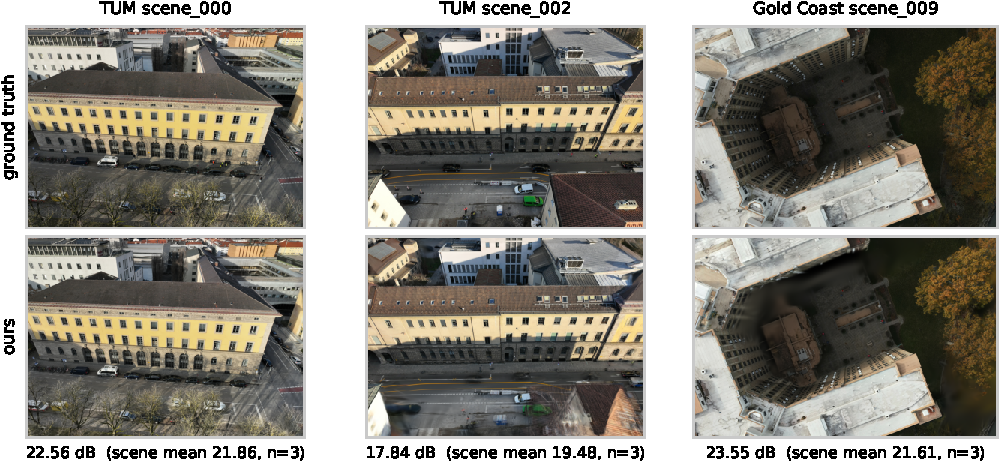
\includegraphics[width=\textwidth]{fig/renders.pdf}
\caption{Qualitative rendering results on held-out views. The top row shows the
released reference images, and the bottom row shows our submitted renders,
obtained by averaging three seeds. Each scene contains three held-out views; we
show the view with median PSNR and report the scene-level mean. Averaging reduces
seed-dependent speckle but does not resolve structural errors: thin foreground
objects and sparsely observed surfaces remain blurred across all seeds. We do not
decompose the rendering metric by error type, so this is qualitative.}
\label{fig:renders}
\end{figure*}

\begin{table*}[t]
\centering\small
\setlength{\tabcolsep}{5pt}
\begin{tabular}{@{}rlrrrrrr@{}}
\toprule
\# & team & Final & PSNR & SSIM & LPIPS & F-score & mIoU 3D \\
\midrule
1 & \code{totototo} & 1.67 & 21.23 & 0.75 & 0.28 & 0.56 & 0.47 \\
2 & \code{lionelsy} & 1.61 & 20.03 & 0.7 & 0.29 & 0.64 & 0.37 \\
3 & \code{windrise} & 1.6 & 19.75 & 0.72 & 0.28 & 0.61 & 0.38 \\
\rowcolor{black!7}
4 & \textbf{\code{kylechen1211}} & 1.53 & 19.95 & 0.72 & 0.29 & 0.58 & 0.34 \\
5 & \code{manish} & 1.48 & 20.9 & 0.74 & 0.3 & 0.64 & 0.22 \\
6 & \code{qqqqyyyyzzzz} & 1.41 & 19.11 & 0.63 & 0.35 & 0.62 & 0.24 \\
7 & \code{qqqyyyzzz} & 1.41 & 19.09 & 0.63 & 0.35 & 0.62 & 0.24 \\
8 & \code{xcyin} & 1.41 & 20.07 & 0.69 & 0.31 & 0.62 & 0.19 \\
9 & \code{tos111} & 1.4 & 21.23 & 0.75 & 0.28 & 0.56 & 0.2 \\
10 & \code{qiuyizhuo} & 1.38 & 18.91 & 0.63 & 0.36 & 0.62 & 0.21 \\
11 & \code{qinwenbin} & 1.36 & 18.54 & 0.55 & 0.35 & 0.57 & 0.26 \\
12 & \code{qwbqwbqwb} & 1.34 & 18.54 & 0.55 & 0.35 & 0.57 & 0.25 \\
13 & \code{yruichen} & 1.3 & 19.86 & 0.67 & 0.4 & 0.6 & 0.15 \\
14 & \code{toscanago} & 1.3 & 21.23 & 0.75 & 0.28 & 0.53 & 0.13 \\
15 & \code{acceon} & 1.29 & 19.22 & 0.58 & 0.39 & 0.46 & 0.3 \\
16 & \code{fxfyhx} & 1.27 & 17.37 & 0.49 & 0.44 & 0.59 & 0.22 \\
17 & \code{hclab} & 1.18 & 18.58 & 0.66 & 0.38 & 0.56 & 0.07 \\
18 & \code{vapaus} & 1.17 & 17.65 & 0.51 & 0.41 & 0.57 & 0.12 \\
19 & \code{zhayi} & 1.11 & 18.17 & 0.65 & 0.37 & 0.48 & 0.09 \\
20 & \code{licheng} & 1.09 & 17.92 & 0.63 & 0.39 & 0.49 & 0.07 \\
21 & \code{y1nnng} & 1.06 & 17.0 & 0.47 & 0.4 & 0.51 & 0.08 \\
\midrule
\multicolumn{2}{@{}l}{median of 21} & 1.36 & 19.11 & 0.65 & 0.35 & 0.57 & 0.22 \\
\bottomrule
\end{tabular}
\caption{The closed final phase in full, all 21 entries, read from the public
endpoint \url{https://www.codabench.org/api/phases/29458/get_leaderboard/} and
kept verbatim beside the factsheet sources. Our row is shaded.}
\label{tab:leaderboard}
\end{table*}

\begin{table}[t]
\centering\small
\setlength{\tabcolsep}{3.4pt}
\begin{tabular}{@{}lcrrrr@{}}
\toprule
phase & rank & Final & PSNR & F & mIoU \\
\midrule
development & 1 of 19 & 1.60 & 19.68 & 0.51 & 0.52 \\
final & 4 of 21 & 1.53 & 19.95 & 0.58 & 0.34 \\
\bottomrule
\end{tabular}
\caption{Our best entry in each phase, same source as \cref{tab:leaderboard}
(development is phase 29457; submission 894488 and 909861). We led the
}
\label{tab:phases}
\end{table}

\begin{figure*}[t]
\centering
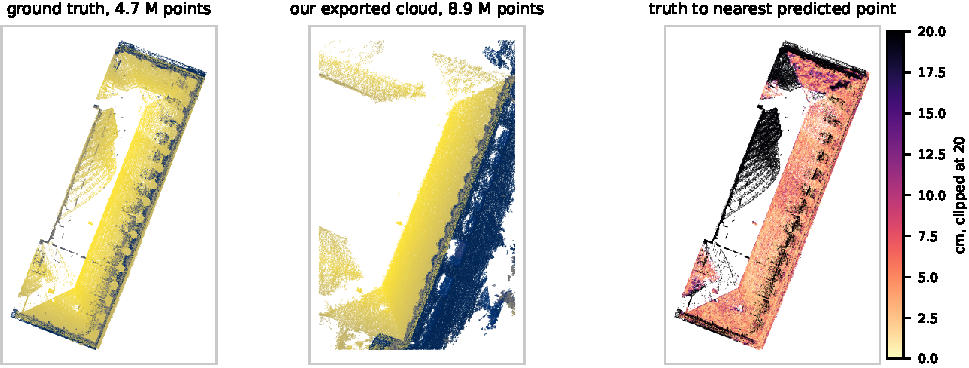
\includegraphics[width=\textwidth]{fig/geometry.pdf}
\caption{The geometry term on \code{tum/scene\_000}, viewed from above. Left:
released ground truth. Middle: the cloud our pipeline exports. Right: the
distance from each ground-truth point to the nearest point we predict, which is
the recall side of the F-score. Both clouds are cropped to the truth's bounding
box and voxel-downsampled at 2\,cm first, exactly as the scorer does. Roof
surfaces sit within a few centimetres;
the dark regions are courtyard and vegetation seen from too few views. This
exported cloud scores $F=0.611$; the copy inside the submitted archive scores
$0.413$, because the archive spends its point budget on the seven scenes the final
phase scores, thinning the six it does not: \code{tum/scene\_000} to
\code{scene\_003} and \code{gold\_coast/scene\_009} and \code{scene\_010}.}
\label{fig:geometry}
\end{figure*}

\begin{figure*}[t]
\centering
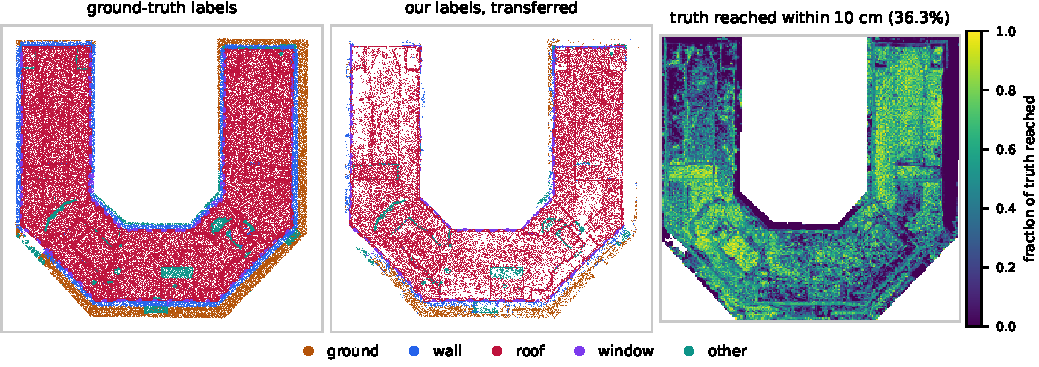
\includegraphics[width=\textwidth]{fig/semantic.pdf}
\caption{The semantic term on \code{gold\_coast/scene\_009}, viewed from above.
Left: released ground-truth labels. Middle: our submitted labels, transferred to
the truth exactly as the metric does. Right: the fraction of ground-truth points
in each cell that have any prediction within 10\,cm. Per-class IoU is
0.220 ground, 0.293 wall, 0.456 roof, 0.244 window and 0.296 other, a mean of
0.302. The third panel is the point of \cref{sec:metric}: \textbf{63.7\% of the
ground truth has nothing of ours within 10\,cm at all}, and every one of those
points is an error the metric charges us.}
\label{fig:semantic}
\end{figure*}

\subsection{Novelty and relation to prior work}
\label{sec:novelty}

Our depth component does not change the 2DGS formulation. It exposes an implicit
requirement of the rendering geometry, provides a patch-free correction for the
gsplat readout, and quantifies its effect on the TwinWorld benchmark. Without
the correction, the native path measures center-depth surrogates rather than the
surface depth defined by 2DGS~\cite{huang2024_2dgs}; the discrepancy also
propagates to gsplat's normal-consistency loss.

The lattice construction in \cref{sec:disclosure} follows
Bambah~\cite{bambah1954}, as presented by Conway and
Sloane~\cite{conway1999sphere}. Alam and Haas~\cite{alam2006coverage} previously
applied optimal covering lattices to sensor coverage and derived the same
constant of 1.859. SparseOcc~\cite{liu2024sparseocc} also showed that thickening
a surface can exploit a one-sided occupancy metric, reporting improvements of
5--15 mIoU. Neither the specific system nor the benchmark analysis
presented in this submission has been published previously.

%---------------------------------------------------------------------------
\section{Ensemble and fusion strategies}

The final submission uses two ensemble strategies.

\textbf{Five-seed agreement filter (geometry).} We train five geometry models
per TUM scene, differing only in random seed. The point cloud fused from seed~0
is filtered by retaining points supported within 5\,cm by at least two of the
remaining four seeds. This operation is an agreement filter rather than a fusion
step, because it adds no points. On the four scenes with released ground truth,
it improves \code{geometry\_score} by 0.029 and removes 28.5\% of points from the
submitted clouds.

\textbf{Three-seed render averaging.} We compute the per-pixel mean of three
rendering models. This improves \code{rendering\_score} by 0.026 and outperforms
the best individual seed on five of the six measurable scenes. Pixel-wise median
aggregation is consistently worse than the mean (0.5979 versus 0.6026), which
fits approximately symmetric seed-to-seed errors.

We also evaluated, but did not submit, a distance-gated floater-pruning strategy.
Although it improved three scenes, its mean effect over 18 paired comparisons
across six scenes and three seeds was $-0.0012$.

%---------------------------------------------------------------------------
\section{Disclosed properties of the submission}
\label{sec:disclosure}

Three properties of the final submission.

\textbf{1. Released development-set ground truth is used to align test point
clouds.} Because \code{scene\_009} and \code{scene\_010} include ground truth,
their frame offsets can be measured directly. Ground truth is unavailable for
\code{scene\_011} and \code{scene\_012}, two of the seven scenes evaluated in the
final phase, so their offsets are inferred. We transfer the offsets measured on
the first two scenes and also transform the ground-truth cloud of
\code{scene\_010} into the camera frame of \code{scene\_011} through a joint
COLMAP reconstruction of the three registrable, partially overlapping Gold Coast
scenes. Two of our submissions isolate the effect: \code{v0.19} and \code{v0.20} differ
only in whether this offset is applied to those two scenes, and scored 1.2010 and
1.27, with PSNR, SSIM, LPIPS and F-score unchanged and the whole difference in
mIoU, 0.1207 to 0.19. We read ``external ground-truth data'' in the challenge
terms as data from outside the release, which this is not; if the intended
reading is stricter, this is the item it applies to. The offset is a single
parameter of the
submission-packing step, and reverting it changes one line.

\textbf{2. One of the three offset estimates uses scores returned for our own
submissions.} We model pooled mIoU as $a\,g(o-t)$, where $g$ is a response curve
measured on the two scenes with released ground truth, and fit $t$ using five of
our scored submissions.

\textbf{3. For \code{scene\_011} and \code{scene\_012}, the submitted point cloud
is a labeled occupancy volume rather than a labeled surface.} This representation
optimizes the stated semantic metric but does not improve reconstruction quality.
It contributes more to our semantic score than any other individual component.
\Cref{fig:volume} visualizes the representation, and \cref{sec:metric} analyzes
the underlying metric behavior independently of our entry.

\begin{figure*}[t]
\centering
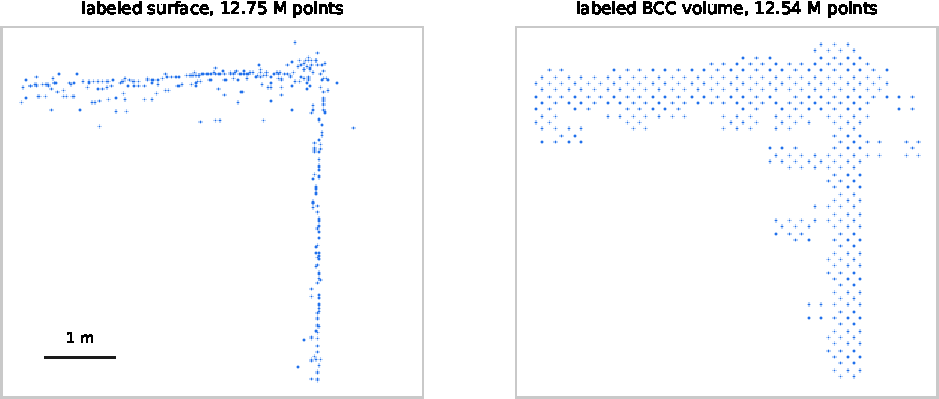
\includegraphics[width=\textwidth]{fig/volume.pdf}
\caption{Visualization of disclosed property~3 using the submitted archives. We
show corresponding $8 \times 5$\,m vertical slices of \code{scene\_011}, each
12\,cm thick. Left: the labeled surface used through submission v0.27. Right:
the body-centered cubic (BCC) occupancy volume in the final submission, using lattice
constant $a=0.19$\,m within a 0.17\,m shell. The point counts are nearly equal;
the representations differ primarily in whether points lie on the surface or
fill its neighborhood. This change improves leaderboard mIoU by 0.06, despite
producing a less faithful
geometric representation; see \cref{sec:metric}.}
\label{fig:volume}
\end{figure*}

%---------------------------------------------------------------------------
\section{Other details}

\subsection{Impressions and practical challenges}

The dataset is well suited to evaluating digital-twin reconstruction, and the
three-part score prevents appearance alone from determining the ranking. The main
practical challenge was model selection under limited supervision: the final
phase evaluates seven scenes without released ground truth, so choices validated
on the six development scenes have to transfer to unseen data. This led to two
notable errors. First, we selected a Gold Coast representation using development
clouds thinned to 12\,cm, whereas the target clouds used 6\,cm spacing; an
improvement factor we expected to be 2.26 was only 1.29 on the leaderboard. Second, one
scene was submitted with approximately one quarter of its spatial extent missing,
and a ground-truth-free diagnostic identified the issue only after three
submissions.

A second difficulty concerns the undocumented point-count limit. Archives above
this limit are rejected with a null exit code and no diagnostic message. We used
three submissions to estimate the threshold. Publishing the limit and returning
an explicit error message would make this failure mode substantially easier to
diagnose.

\subsection{Comments on the evaluation metric}
\label{sec:metric}

We identify one property of the semantic score that may merit attention in future
editions.

The Gold Coast semantic metric performs a ground-truth-driven nearest-neighbor
lookup within 10\,cm and contains no precision term: a predicted point with no
nearby ground-truth point incurs no penalty. On the two scenes with released
ground truth, removing every false positive from our submission increases pooled
mIoU from 0.3104 to 0.3207. In contrast, matching every ground-truth point while
retaining our assigned labels would increase mIoU to 0.94. \Cref{fig:semantic} shows both halves of this on one scene: our labels beside
the truth, and how much of the truth we are near enough to label at all. Under
this analysis, the metric is approximately 60 times more sensitive to coverage
than to
precision.

Under this scoring rule, a labeled occupancy volume can be preferable to a
surface representation. The optimization then becomes a covering problem: place
$N$ points to maximize the proportion of ground-truth points within 10\,cm of a
prediction. We use a body-centered cubic lattice, the lowest-density
\emph{lattice} covering of three-dimensional space~\cite{bambah1954,conway1999sphere}.
It guarantees a 10\,cm match using 349 points per cubic meter, compared with 649
for a simple cubic grid.

\begin{figure}[t]
\centering
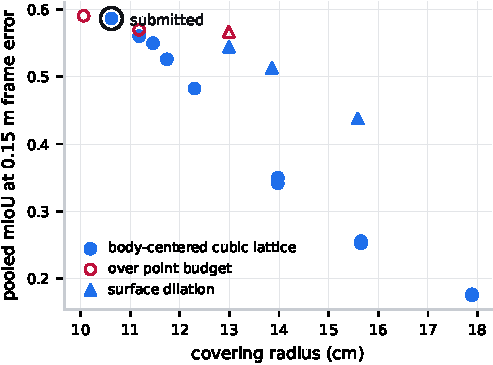
\includegraphics[width=\linewidth]{fig/sweep.pdf}
\caption{The lattice sweep. Each point is one construction of the Gold Coast
cloud, scored on the two scenes that ship ground truth. Filled markers are
inside the per-cloud point budget that has already been accepted by the
evaluator; open red markers exceed it. Within the lattice family the score
tracks the covering radius and is nearly indifferent to shell thickness, which
is why the submitted configuration is the smallest admissible radius rather than
the thickest shell. The surface-dilation variants are a different construction
and are not comparable to the lattices at equal radius; see the text.}
\label{fig:sweep}
\end{figure}

\Cref{fig:sweep} is the sweep behind that choice. Of the 29 constructions run,
the 19 whose lattice has a defined covering radius are plotted, scored on
the two Gold Coast scenes that ship ground truth at the residual frame error the
offset correction is expected to leave, with the selection criterion fixed before
the grid ran. Two things in it are worth separating.

Within the lattice family the score is governed by the covering radius and
almost nothing else. It falls monotonically from 0.587 at a radius of 10.6\,cm
to 0.177 at 17.9\,cm, while the covered volume stays within
36{,}000--51{,}000\,m$^3$. Shell thickness barely registers: at a radius of
15.7\,cm, tripling the shell from 0.45 to 0.75\,m moves the score from 0.2523 to
0.2556, and the three shells tried at 14.0\,cm all land within 0.008 of each
other. We had expected a coarser lattice to buy back its loss through thickness,
and it does not.

The comparison does not carry across constructions, and \cref{fig:sweep}
separates them for that reason. The surface-dilation variants, which thicken the
reconstructed surface instead of filling space, sit above the lattice trend at
equal covering radius: a dilation at 13.0\,cm scores 0.545 where a lattice at
12.3\,cm scores 0.483. They place points only where the surface already is,
which is a real advantage that covering radius alone does not express. What the
lattice buys is the guarantee, not a uniformly better score at every budget.

The covered volume remains within
36{,}000--51{,}000\,m$^3$, while the score varies by a factor of three. This
indicates that point placement, rather than total covered volume, governs the
metric. An oracle with access to ground truth matches the lattice score using 17
times fewer points, suggesting that the point budget is not the limiting factor;
approximately 30\% of ground-truth points are not close to any reconstructed
surface.

\textbf{Comparison with related benchmarks.} KITTI-360 uses a similar
ground-truth-driven nearest-neighbor label-transfer metric for semantic
mapping~\cite{liao2022kitti360}. However, it also reports geometric accuracy for
the same predicted points, so dilating a point cloud degrades its geometric
score. ScanNet-family benchmarks evaluate predictions on a provided point set;
consequently, predictions correspond to ground-truth points and false positives
are counted directly. In TwinWorld, \code{geometry\_score} is evaluated on TUM
scenes and \code{semantic\_score} on a disjoint set of Gold Coast scenes. The
combined score therefore does not penalize volumetric predictions on the scenes
used for semantic evaluation. We recommend addressing this cross-scene
decoupling rather than changing the mIoU definition itself.

\subsection{Suggestions for future editions}

\begin{enumerate}[1.]\itemsep2pt
\item \textbf{Add a precision component to semantic evaluation and evaluate it
      on the same scenes as geometry.} This follows the surface evaluation of
      Tanks and Temples~\cite{knapitsch2017tanks} and the paired semantic and
      geometric reporting of KITTI-360~\cite{liao2022kitti360}, and would remove
      the incentive for volumetric predictions.
\item \textbf{Publish the point-count limit and report an explicit error when it
      is exceeded.} This would prevent teams from spending submissions solely to
      diagnose an undocumented constraint.
\item \textbf{Reassess the reliability of the 5\,cm threshold.} The TUM2TWIN
      data-quality analysis~\cite[Tab.~2]{wysocki2026tum2twin} reports absolute
      and relative accuracies of 0.08\,m and 0.05\,m, respectively, for the
      uncrewed aerial system (UAS) laser scan. UseGeo~\cite{nex2023usegeo}
      reports a mean cloud-to-cloud error of 8.5\,cm for conventional dense
      photogrammetry relative to an airborne light detection and ranging (LiDAR)
      survey, using 224 images and at least eight rays per object point. With only
      12--24 views, F-score at 5\,cm may partly reflect uncertainty in the
      reference data. We present this as a question because we have not directly
      measured reference accuracy.
\item \textbf{Release ground truth for one withheld scene after the challenge
      closes.} This would enable teams to assess how design choices transfer from
      the six development scenes to the seven held-out scenes.
\item \textbf{State whether development-set ground truth may inform test-set
      predictions.} The Gold Coast georeferencing offset makes this distinction
      consequential, but the current terms do not resolve it explicitly.
\end{enumerate}

\subsection{Limitations of the released checkpoints}

The 39 rendering runs were executed without checkpoint saving; consequently, the
Gaussian parameters that produced the submitted images are unavailable. We
tested whether deterministic retraining could recover them. Two runs using
identical commands, random seeds, and GPUs differed by 31{,}224 Gaussians at
termination; none of their three rendered frames were byte-identical, and the
PSNR between corresponding runs ranged from 15.7 to 23.8\,dB. The training code
seeds only the framework's global random number generator, while the gsplat
backward pass accumulates gradients atomically, in an order that is not fixed
between launches.

The results bundle therefore contains every rendered image from all three seeds,
the 39 averaged images that are byte-identical to the submitted archive, and the
complete configuration and metrics for each run. We do not provide retrained
weights as substitutes for the original checkpoints. Checkpoints are available
for every submitted point cloud except seed~0 of \code{tum/scene\_006}, which was
also trained without checkpoint saving. Its remaining four agreement-filtering
seeds, exported point cloud, color data, and generation receipt are included.

\section*{Acknowledgements}

We thank the National Center for High-performance Computing (NCHC), Taiwan, for
the computational and storage resources used in this work, under project
\code{GOV114009}.

{\small
\bibliographystyle{ieeenat_fullname}
\bibliography{egbib}
}

\end{document}
